\documentclass[1p]{elsarticle_modified}
%\bibliographystyle{elsarticle-num}

%\usepackage[colorlinks]{hyperref}
%\usepackage{abbrmath_seonhwa} %\Abb, \Ascr, \Acal ,\Abf, \Afrak
\usepackage{amsfonts}
\usepackage{amssymb}
\usepackage{amsmath}
\usepackage{amsthm}
\usepackage{scalefnt}
\usepackage{amsbsy}
\usepackage{kotex}
\usepackage{caption}
\usepackage{subfig}
\usepackage{color}
\usepackage{graphicx}
\usepackage{xcolor} %% white, black, red, green, blue, cyan, magenta, yellow
\usepackage{float}
\usepackage{setspace}
\usepackage{hyperref}

\usepackage{tikz}
\usetikzlibrary{arrows}

\usepackage{multirow}
\usepackage{array} % fixed length table
\usepackage{hhline}

%%%%%%%%%%%%%%%%%%%%%
\makeatletter
\renewcommand*\env@matrix[1][\arraystretch]{%
	\edef\arraystretch{#1}%
	\hskip -\arraycolsep
	\let\@ifnextchar\new@ifnextchar
	\array{*\c@MaxMatrixCols c}}
\makeatother %https://tex.stackexchange.com/questions/14071/how-can-i-increase-the-line-spacing-in-a-matrix
%%%%%%%%%%%%%%%

\usepackage[normalem]{ulem}

\newcommand{\msout}[1]{\ifmmode\text{\sout{\ensuremath{#1}}}\else\sout{#1}\fi}
%SOURCE: \msout is \stkout macro in https://tex.stackexchange.com/questions/20609/strikeout-in-math-mode

\newcommand{\cancel}[1]{
	\ifmmode
	{\color{red}\msout{#1}}
	\else
	{\color{red}\sout{#1}}
	\fi
}

\newcommand{\add}[1]{
	{\color{blue}\uwave{#1}}
}

\newcommand{\replace}[2]{
	\ifmmode
	{\color{red}\msout{#1}}{\color{blue}\uwave{#2}}
	\else
	{\color{red}\sout{#1}}{\color{blue}\uwave{#2}}
	\fi
}

\newcommand{\Sol}{\mathcal{S}} %segment
\newcommand{\D}{D} %diagram
\newcommand{\A}{\mathcal{A}} %arc


%%%%%%%%%%%%%%%%%%%%%%%%%%%%%5 test

\def\sl{\operatorname{\textup{SL}}(2,\Cbb)}
\def\psl{\operatorname{\textup{PSL}}(2,\Cbb)}
\def\quan{\mkern 1mu \triangleright \mkern 1mu}

\theoremstyle{definition}
\newtheorem{thm}{Theorem}[section]
\newtheorem{prop}[thm]{Proposition}
\newtheorem{lem}[thm]{Lemma}
\newtheorem{ques}[thm]{Question}
\newtheorem{cor}[thm]{Corollary}
\newtheorem{defn}[thm]{Definition}
\newtheorem{exam}[thm]{Example}
\newtheorem{rmk}[thm]{Remark}
\newtheorem{alg}[thm]{Algorithm}

\newcommand{\I}{\sqrt{-1}}
\begin{document}

%\begin{frontmatter}
%
%\title{Boundary parabolic representations of knots up to 8 crossings}
%
%%% Group authors per affiliation:
%\author{Yunhi Cho} 
%\address{Department of Mathematics, University of Seoul, Seoul, Korea}
%\ead{yhcho@uos.ac.kr}
%
%
%\author{Seonhwa Kim} %\fnref{s_kim}}
%\address{Center for Geometry and Physics, Institute for Basic Science, Pohang, 37673, Korea}
%\ead{ryeona17@ibs.re.kr}
%
%\author{Hyuk Kim}
%\address{Department of Mathematical Sciences, Seoul National University, Seoul 08826, Korea}
%\ead{hyukkim@snu.ac.kr}
%
%\author{Seokbeom Yoon}
%\address{Department of Mathematical Sciences, Seoul National University, Seoul, 08826,  Korea}
%\ead{sbyoon15@snu.ac.kr}
%
%\begin{abstract}
%We find all boundary parabolic representation of knots up to 8 crossings.
%
%\end{abstract}
%\begin{keyword}
%    \MSC[2010] 57M25 
%\end{keyword}
%
%\end{frontmatter}

%\linenumbers
%\tableofcontents
%
\newcommand\colored[1]{\textcolor{white}{\rule[-0.35ex]{0.8em}{1.4ex}}\kern-0.8em\color{red} #1}%
%\newcommand\colored[1]{\textcolor{white}{ #1}\kern-2.17ex	\textcolor{white}{ #1}\kern-1.81ex	\textcolor{white}{ #1}\kern-2.15ex\color{red}#1	}

{\Large $\underline{11n_{62}~(K11n_{62})}$}

\setlength{\tabcolsep}{10pt}
\renewcommand{\arraystretch}{1.6}
\vspace{1cm}\begin{tabular}{m{100pt}>{\centering\arraybackslash}m{274pt}}
\multirow{5}{120pt}{
	\centering
	\includegraphics[width=112pt]{../../../GIT/diagram.site/Diagrams/png/678_11n_62.png}\\
\ \ \ A knot diagram\footnotemark}&
\allowdisplaybreaks
\textbf{Linearized knot diagam} \\
\cline{2-2}
 &
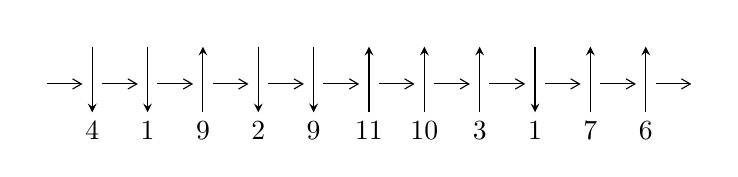
\begin{tikzpicture}[x=20pt, y=17pt]
	% nodes
	\node (C0) at (0, 0) {};
	\node (C1) at (1, 0) {};
	\node (C1U) at (1, +1) {};
	\node (C1D) at (1, -1) {4};

	\node (C2) at (2, 0) {};
	\node (C2U) at (2, +1) {};
	\node (C2D) at (2, -1) {1};

	\node (C3) at (3, 0) {};
	\node (C3U) at (3, +1) {};
	\node (C3D) at (3, -1) {9};

	\node (C4) at (4, 0) {};
	\node (C4U) at (4, +1) {};
	\node (C4D) at (4, -1) {2};

	\node (C5) at (5, 0) {};
	\node (C5U) at (5, +1) {};
	\node (C5D) at (5, -1) {9};

	\node (C6) at (6, 0) {};
	\node (C6U) at (6, +1) {};
	\node (C6D) at (6, -1) {11};

	\node (C7) at (7, 0) {};
	\node (C7U) at (7, +1) {};
	\node (C7D) at (7, -1) {10};

	\node (C8) at (8, 0) {};
	\node (C8U) at (8, +1) {};
	\node (C8D) at (8, -1) {3};

	\node (C9) at (9, 0) {};
	\node (C9U) at (9, +1) {};
	\node (C9D) at (9, -1) {1};

	\node (C10) at (10, 0) {};
	\node (C10U) at (10, +1) {};
	\node (C10D) at (10, -1) {7};

	\node (C11) at (11, 0) {};
	\node (C11U) at (11, +1) {};
	\node (C11D) at (11, -1) {6};
	\node (C12) at (12, 0) {};

	% arrows
	\draw[->,>={angle 60}]
	(C0) edge (C1) (C1) edge (C2) (C2) edge (C3) (C3) edge (C4) (C4) edge (C5) (C5) edge (C6) (C6) edge (C7) (C7) edge (C8) (C8) edge (C9) (C9) edge (C10) (C10) edge (C11) (C11) edge (C12) ;	\draw[->,>=stealth]
	(C1U) edge (C1D) (C2U) edge (C2D) (C3D) edge (C3U) (C4U) edge (C4D) (C5U) edge (C5D) (C6D) edge (C6U) (C7D) edge (C7U) (C8D) edge (C8U) (C9U) edge (C9D) (C10D) edge (C10U) (C11D) edge (C11U) ;
	\end{tikzpicture} \\
\hhline{~~} \\& 
\textbf{Solving Sequence} \\ \cline{2-2} 
 &
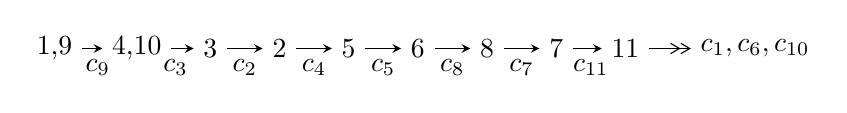
\begin{tikzpicture}[x=25pt, y=7pt]
	% node
	\node (A0) at (-1/8, 0) {1,9};
	\node (A1) at (17/16, 0) {4,10};
	\node (A2) at (17/8, 0) {3};
	\node (A3) at (25/8, 0) {2};
	\node (A4) at (33/8, 0) {5};
	\node (A5) at (41/8, 0) {6};
	\node (A6) at (49/8, 0) {8};
	\node (A7) at (57/8, 0) {7};
	\node (A8) at (65/8, 0) {11};
	\node (C1) at (1/2, -1) {$c_{9}$};
	\node (C2) at (13/8, -1) {$c_{3}$};
	\node (C3) at (21/8, -1) {$c_{2}$};
	\node (C4) at (29/8, -1) {$c_{4}$};
	\node (C5) at (37/8, -1) {$c_{5}$};
	\node (C6) at (45/8, -1) {$c_{8}$};
	\node (C7) at (53/8, -1) {$c_{7}$};
	\node (C8) at (61/8, -1) {$c_{11}$};
	\node (A9) at (10, 0) {$c_{1},c_{6},c_{10}$};

	% edge
	\draw[->,>=stealth]	
	(A0) edge (A1) (A1) edge (A2) (A2) edge (A3) (A3) edge (A4) (A4) edge (A5) (A5) edge (A6) (A6) edge (A7) (A7) edge (A8) ;
	\draw[->>,>={angle 60}]	
	(A8) edge (A9);
\end{tikzpicture} \\ 

\end{tabular} \\

\footnotetext{
The image of knot diagram is generated by the software ``\textbf{Draw programme}" developed by Andrew Bartholomew(\url{http://www.layer8.co.uk/maths/draw/index.htm\#Running-draw}), where we modified some parts for our purpose(\url{https://github.com/CATsTAILs/LinksPainter}).
}\phantom \\ \newline 
\centering \textbf{Ideals for irreducible components\footnotemark of $X_{\text{par}}$} 
 
\begin{align*}
I^u_{1}&=\langle 
2464615243943 u^{19}+4244123981661 u^{18}+\cdots+9728979932592 b+197070286033,\\
\phantom{I^u_{1}}&\phantom{= \langle  }-5509715115239 u^{19}-10822359944445 u^{18}+\cdots+9728979932592 a+3267475985807,\\
\phantom{I^u_{1}}&\phantom{= \langle  }u^{20}+2 u^{19}+\cdots+5 u^2+1\rangle \\
I^u_{2}&=\langle 
b,\;- u^3- u^2+a- u,\;u^4+u^3+u^2+1\rangle \\
\\
\end{align*}
\raggedright * 2 irreducible components of $\dim_{\mathbb{C}}=0$, with total 24 representations.\\
\footnotetext{All coefficients of polynomials are rational numbers. But the coefficients are sometimes approximated in decimal forms when there is not enough margin.}
\newpage
\renewcommand{\arraystretch}{1}
\centering \section*{I. $I^u_{1}= \langle 2.46\times10^{12} u^{19}+4.24\times10^{12} u^{18}+\cdots+9.73\times10^{12} b+1.97\times10^{11},\;-5.51\times10^{12} u^{19}-1.08\times10^{13} u^{18}+\cdots+9.73\times10^{12} a+3.27\times10^{12},\;u^{20}+2 u^{19}+\cdots+5 u^2+1 \rangle$}
\flushleft \textbf{(i) Arc colorings}\\
\begin{tabular}{m{7pt} m{180pt} m{7pt} m{180pt} }
\flushright $a_{1}=$&$\begin{pmatrix}0\\u\end{pmatrix}$ \\
\flushright $a_{9}=$&$\begin{pmatrix}1\\0\end{pmatrix}$ \\
\flushright $a_{4}=$&$\begin{pmatrix}0.566320 u^{19}+1.11238 u^{18}+\cdots+2.54326 u-0.335850\\-0.253327 u^{19}-0.436235 u^{18}+\cdots+1.56632 u-0.0202560\end{pmatrix}$ \\
\flushright $a_{10}=$&$\begin{pmatrix}1\\u^2\end{pmatrix}$ \\
\flushright $a_{3}=$&$\begin{pmatrix}0.819647 u^{19}+1.54862 u^{18}+\cdots+0.976937 u-0.315594\\-0.253327 u^{19}-0.436235 u^{18}+\cdots+1.56632 u-0.0202560\end{pmatrix}$ \\
\flushright $a_{2}=$&$\begin{pmatrix}0.819647 u^{19}+1.54862 u^{18}+\cdots+0.976937 u-0.315594\\-0.396913 u^{19}-0.728464 u^{18}+\cdots+2.38597 u-0.110931\end{pmatrix}$ \\
\flushright $a_{5}=$&$\begin{pmatrix}-0.650241 u^{19}-1.16470 u^{18}+\cdots+2.95229 u-0.131187\\0.105052 u^{19}+0.296152 u^{18}+\cdots-1.03621 u+0.246713\end{pmatrix}$ \\
\flushright $a_{6}=$&$\begin{pmatrix}-0.755292 u^{19}-1.46085 u^{18}+\cdots+3.98849 u-0.377900\\0.105052 u^{19}+0.296152 u^{18}+\cdots-1.03621 u+0.246713\end{pmatrix}$ \\
\flushright $a_{8}=$&$\begin{pmatrix}-0.246713 u^{19}-0.388373 u^{18}+\cdots-0.520256 u-1.03621\\0.135781 u^{19}+0.563424 u^{18}+\cdots-0.131187 u+0.650241\end{pmatrix}$ \\
\flushright $a_{7}=$&$\begin{pmatrix}-0.296445 u^{19}-0.863365 u^{18}+\cdots-0.142357 u-1.79150\\0.253735 u^{19}+0.918450 u^{18}+\cdots-0.0814545 u+1.02577\end{pmatrix}$ \\
\flushright $a_{11}=$&$\begin{pmatrix}-0.408108 u^{19}-0.952751 u^{18}+\cdots+1.33641 u-1.23004\\-0.300860 u^{19}-0.485772 u^{18}+\cdots-0.821932 u+0.544643\end{pmatrix}$\\ \flushright $a_{11}=$&$\begin{pmatrix}-0.408108 u^{19}-0.952751 u^{18}+\cdots+1.33641 u-1.23004\\-0.300860 u^{19}-0.485772 u^{18}+\cdots-0.821932 u+0.544643\end{pmatrix}$\\&\end{tabular}
\flushleft \textbf{(ii) Obstruction class $= -1$}\\~\\
\flushleft \textbf{(iii) Cusp Shapes $= \frac{815395233485}{405374163858} u^{19}+\frac{427506532937}{135124721286} u^{18}+\cdots-\frac{421979351069}{405374163858} u-\frac{2038924430399}{405374163858}$}\\~\\
\newpage\renewcommand{\arraystretch}{1}
\flushleft \textbf{(iv) u-Polynomials at the component}\newline \\
\begin{tabular}{m{50pt}|m{274pt}}
Crossings & \hspace{64pt}u-Polynomials at each crossing \\
\hline $$\begin{aligned}c_{1},c_{4}\end{aligned}$$&$\begin{aligned}
&u^{20}-5 u^{19}+\cdots-4 u+1
\end{aligned}$\\
\hline $$\begin{aligned}c_{2}\end{aligned}$$&$\begin{aligned}
&u^{20}+3 u^{19}+\cdots-4 u+1
\end{aligned}$\\
\hline $$\begin{aligned}c_{3},c_{8}\end{aligned}$$&$\begin{aligned}
&u^{20}- u^{19}+\cdots-8 u+16
\end{aligned}$\\
\hline $$\begin{aligned}c_{5}\end{aligned}$$&$\begin{aligned}
&u^{20}+2 u^{19}+\cdots+154 u+445
\end{aligned}$\\
\hline $$\begin{aligned}c_{6},c_{7},c_{10}\\c_{11}\end{aligned}$$&$\begin{aligned}
&u^{20}+2 u^{19}+\cdots+2 u+1
\end{aligned}$\\
\hline $$\begin{aligned}c_{9}\end{aligned}$$&$\begin{aligned}
&u^{20}-2 u^{19}+\cdots+5 u^2+1
\end{aligned}$\\
\hline
\end{tabular}\\~\\
\newpage\renewcommand{\arraystretch}{1}
\flushleft \textbf{(v) Riley Polynomials at the component}\newline \\
\begin{tabular}{m{50pt}|m{274pt}}
Crossings & \hspace{64pt}Riley Polynomials at each crossing \\
\hline $$\begin{aligned}c_{1},c_{4}\end{aligned}$$&$\begin{aligned}
&y^{20}-3 y^{19}+\cdots+4 y+1
\end{aligned}$\\
\hline $$\begin{aligned}c_{2}\end{aligned}$$&$\begin{aligned}
&y^{20}+33 y^{19}+\cdots+4 y+1
\end{aligned}$\\
\hline $$\begin{aligned}c_{3},c_{8}\end{aligned}$$&$\begin{aligned}
&y^{20}-27 y^{19}+\cdots-1344 y+256
\end{aligned}$\\
\hline $$\begin{aligned}c_{5}\end{aligned}$$&$\begin{aligned}
&y^{20}+38 y^{19}+\cdots+4809874 y+198025
\end{aligned}$\\
\hline $$\begin{aligned}c_{6},c_{7},c_{10}\\c_{11}\end{aligned}$$&$\begin{aligned}
&y^{20}+22 y^{19}+\cdots+10 y+1
\end{aligned}$\\
\hline $$\begin{aligned}c_{9}\end{aligned}$$&$\begin{aligned}
&y^{20}+26 y^{19}+\cdots+10 y+1
\end{aligned}$\\
\hline
\end{tabular}\\~\\
\newpage\flushleft \textbf{(vi) Complex Volumes and Cusp Shapes}
$$\begin{array}{c|c|c}  
\text{Solutions to }I^u_{1}& \I (\text{vol} + \sqrt{-1}CS) & \text{Cusp shape}\\
 \hline 
\begin{aligned}
u &= \phantom{-}0.673071 + 0.753931 I \\
a &= \phantom{-}0.535459 - 0.003526 I \\
b &= \phantom{-}0.731278 + 0.210088 I\end{aligned}
 & \phantom{-}0.02154 - 2.08472 I & \phantom{-}2.36846 + 5.36236 I \\ \hline\begin{aligned}
u &= \phantom{-}0.673071 - 0.753931 I \\
a &= \phantom{-}0.535459 + 0.003526 I \\
b &= \phantom{-}0.731278 - 0.210088 I\end{aligned}
 & \phantom{-}0.02154 + 2.08472 I & \phantom{-}2.36846 - 5.36236 I \\ \hline\begin{aligned}
u &= -0.094946 + 0.739352 I \\
a &= \phantom{-}1.098280 + 0.336321 I \\
b &= \phantom{-}0.448296 + 1.074360 I\end{aligned}
 & -4.77753 + 2.99094 I & -0.69176 - 3.46155 I \\ \hline\begin{aligned}
u &= -0.094946 - 0.739352 I \\
a &= \phantom{-}1.098280 - 0.336321 I \\
b &= \phantom{-}0.448296 - 1.074360 I\end{aligned}
 & -4.77753 - 2.99094 I & -0.69176 + 3.46155 I \\ \hline\begin{aligned}
u &= -0.177522 + 0.687359 I \\
a &= -0.716990 + 0.247004 I \\
b &= -0.553957 + 0.621299 I\end{aligned}
 & \phantom{-}0.995000 - 0.993446 I & \phantom{-}5.17867 + 4.04800 I \\ \hline\begin{aligned}
u &= -0.177522 - 0.687359 I \\
a &= -0.716990 - 0.247004 I \\
b &= -0.553957 - 0.621299 I\end{aligned}
 & \phantom{-}0.995000 + 0.993446 I & \phantom{-}5.17867 - 4.04800 I \\ \hline\begin{aligned}
u &= -1.12972 + 0.93010 I \\
a &= -0.456176 - 0.088007 I \\
b &= -0.757198 + 0.007629 I\end{aligned}
 & -7.51526 + 3.82239 I & \phantom{-}0.11541 - 4.60594 I \\ \hline\begin{aligned}
u &= -1.12972 - 0.93010 I \\
a &= -0.456176 + 0.088007 I \\
b &= -0.757198 - 0.007629 I\end{aligned}
 & -7.51526 - 3.82239 I & \phantom{-}0.11541 + 4.60594 I \\ \hline\begin{aligned}
u &= -0.382707 + 0.237846 I \\
a &= \phantom{-}2.61545 + 0.82402 I \\
b &= -0.767833 + 0.639917 I\end{aligned}
 & -7.81656 + 1.26535 I & -3.51291 - 0.02866 I \\ \hline\begin{aligned}
u &= -0.382707 - 0.237846 I \\
a &= \phantom{-}2.61545 - 0.82402 I \\
b &= -0.767833 - 0.639917 I\end{aligned}
 & -7.81656 - 1.26535 I & -3.51291 + 0.02866 I\\
 \hline 
 \end{array}$$\newpage$$\begin{array}{c|c|c}  
\text{Solutions to }I^u_{1}& \I (\text{vol} + \sqrt{-1}CS) & \text{Cusp shape}\\
 \hline 
\begin{aligned}
u &= \phantom{-}0.18268 + 1.66062 I \\
a &= \phantom{-}0.734667 - 0.455842 I \\
b &= \phantom{-}1.90756 - 0.02696 I\end{aligned}
 & \phantom{-}3.14125 + 1.95377 I & -0.018441 - 0.726692 I \\ \hline\begin{aligned}
u &= \phantom{-}0.18268 - 1.66062 I \\
a &= \phantom{-}0.734667 + 0.455842 I \\
b &= \phantom{-}1.90756 + 0.02696 I\end{aligned}
 & \phantom{-}3.14125 - 1.95377 I & -0.018441 + 0.726692 I \\ \hline\begin{aligned}
u &= \phantom{-}0.177052 + 0.214813 I \\
a &= -2.67119 + 2.37138 I \\
b &= \phantom{-}0.317909 + 0.453091 I\end{aligned}
 & -1.76070 - 0.62769 I & -5.52555 - 1.68478 I \\ \hline\begin{aligned}
u &= \phantom{-}0.177052 - 0.214813 I \\
a &= -2.67119 - 2.37138 I \\
b &= \phantom{-}0.317909 - 0.453091 I\end{aligned}
 & -1.76070 + 0.62769 I & -5.52555 + 1.68478 I \\ \hline\begin{aligned}
u &= -0.21357 + 1.74539 I \\
a &= -0.684239 - 0.489378 I \\
b &= -1.90198 - 0.23325 I\end{aligned}
 & \phantom{-}9.48767 + 1.51858 I & \phantom{-}3.11046 + 0.47571 I \\ \hline\begin{aligned}
u &= -0.21357 - 1.74539 I \\
a &= -0.684239 + 0.489378 I \\
b &= -1.90198 + 0.23325 I\end{aligned}
 & \phantom{-}9.48767 - 1.51858 I & \phantom{-}3.11046 - 0.47571 I \\ \hline\begin{aligned}
u &= \phantom{-}0.24322 + 1.81257 I \\
a &= \phantom{-}0.640240 - 0.509585 I \\
b &= \phantom{-}1.85951 - 0.39598 I\end{aligned}
 & \phantom{-}9.21922 - 6.23574 I & \phantom{-}2.42777 + 5.05678 I \\ \hline\begin{aligned}
u &= \phantom{-}0.24322 - 1.81257 I \\
a &= \phantom{-}0.640240 + 0.509585 I \\
b &= \phantom{-}1.85951 + 0.39598 I\end{aligned}
 & \phantom{-}9.21922 + 6.23574 I & \phantom{-}2.42777 - 5.05678 I \\ \hline\begin{aligned}
u &= -0.27754 + 1.87563 I \\
a &= -0.595500 - 0.521593 I \\
b &= -1.78359 - 0.53915 I\end{aligned}
 & \phantom{-}2.29524 + 9.61446 I & -0.95211 - 4.92599 I \\ \hline\begin{aligned}
u &= -0.27754 - 1.87563 I \\
a &= -0.595500 + 0.521593 I \\
b &= -1.78359 + 0.53915 I\end{aligned}
 & \phantom{-}2.29524 - 9.61446 I & -0.95211 + 4.92599 I\\
 \hline 
 \end{array}$$\newpage\newpage\renewcommand{\arraystretch}{1}
\centering \section*{II. $I^u_{2}= \langle b,\;- u^3- u^2+a- u,\;u^4+u^3+u^2+1 \rangle$}
\flushleft \textbf{(i) Arc colorings}\\
\begin{tabular}{m{7pt} m{180pt} m{7pt} m{180pt} }
\flushright $a_{1}=$&$\begin{pmatrix}0\\u\end{pmatrix}$ \\
\flushright $a_{9}=$&$\begin{pmatrix}1\\0\end{pmatrix}$ \\
\flushright $a_{4}=$&$\begin{pmatrix}u^3+u^2+u\\0\end{pmatrix}$ \\
\flushright $a_{10}=$&$\begin{pmatrix}1\\u^2\end{pmatrix}$ \\
\flushright $a_{3}=$&$\begin{pmatrix}u^3+u^2+u\\0\end{pmatrix}$ \\
\flushright $a_{2}=$&$\begin{pmatrix}u^3+u^2+u\\u\end{pmatrix}$ \\
\flushright $a_{5}=$&$\begin{pmatrix}0\\- u\end{pmatrix}$ \\
\flushright $a_{6}=$&$\begin{pmatrix}u\\- u\end{pmatrix}$ \\
\flushright $a_{8}=$&$\begin{pmatrix}1\\0\end{pmatrix}$ \\
\flushright $a_{7}=$&$\begin{pmatrix}u^2+1\\- u^3- u^2-1\end{pmatrix}$ \\
\flushright $a_{11}=$&$\begin{pmatrix}- u^3\\u^3+u\end{pmatrix}$\\ \flushright $a_{11}=$&$\begin{pmatrix}- u^3\\u^3+u\end{pmatrix}$\\&\end{tabular}
\flushleft \textbf{(ii) Obstruction class $= 1$}\\~\\
\flushleft \textbf{(iii) Cusp Shapes $= 4 u^2+5 u-1$}\\~\\
\newpage\renewcommand{\arraystretch}{1}
\flushleft \textbf{(iv) u-Polynomials at the component}\newline \\
\begin{tabular}{m{50pt}|m{274pt}}
Crossings & \hspace{64pt}u-Polynomials at each crossing \\
\hline $$\begin{aligned}c_{1}\end{aligned}$$&$\begin{aligned}
&(u-1)^4
\end{aligned}$\\
\hline $$\begin{aligned}c_{2},c_{4}\end{aligned}$$&$\begin{aligned}
&(u+1)^4
\end{aligned}$\\
\hline $$\begin{aligned}c_{3},c_{8}\end{aligned}$$&$\begin{aligned}
&u^4
\end{aligned}$\\
\hline $$\begin{aligned}c_{5},c_{9}\end{aligned}$$&$\begin{aligned}
&u^4+u^3+u^2+1
\end{aligned}$\\
\hline $$\begin{aligned}c_{6},c_{7}\end{aligned}$$&$\begin{aligned}
&u^4+u^3+3 u^2+2 u+1
\end{aligned}$\\
\hline $$\begin{aligned}c_{10},c_{11}\end{aligned}$$&$\begin{aligned}
&u^4- u^3+3 u^2-2 u+1
\end{aligned}$\\
\hline
\end{tabular}\\~\\
\newpage\renewcommand{\arraystretch}{1}
\flushleft \textbf{(v) Riley Polynomials at the component}\newline \\
\begin{tabular}{m{50pt}|m{274pt}}
Crossings & \hspace{64pt}Riley Polynomials at each crossing \\
\hline $$\begin{aligned}c_{1},c_{2},c_{4}\end{aligned}$$&$\begin{aligned}
&(y-1)^4
\end{aligned}$\\
\hline $$\begin{aligned}c_{3},c_{8}\end{aligned}$$&$\begin{aligned}
&y^4
\end{aligned}$\\
\hline $$\begin{aligned}c_{5},c_{9}\end{aligned}$$&$\begin{aligned}
&y^4+y^3+3 y^2+2 y+1
\end{aligned}$\\
\hline $$\begin{aligned}c_{6},c_{7},c_{10}\\c_{11}\end{aligned}$$&$\begin{aligned}
&y^4+5 y^3+7 y^2+2 y+1
\end{aligned}$\\
\hline
\end{tabular}\\~\\
\newpage\flushleft \textbf{(vi) Complex Volumes and Cusp Shapes}
$$\begin{array}{c|c|c}  
\text{Solutions to }I^u_{2}& \I (\text{vol} + \sqrt{-1}CS) & \text{Cusp shape}\\
 \hline 
\begin{aligned}
u &= \phantom{-}0.351808 + 0.720342 I \\
a &= -0.547424 + 1.120870 I \\
b &= \phantom{-0.000000 } 0\end{aligned}
 & -1.43393 - 1.41510 I & -0.82145 + 5.62908 I \\ \hline\begin{aligned}
u &= \phantom{-}0.351808 - 0.720342 I \\
a &= -0.547424 - 1.120870 I \\
b &= \phantom{-0.000000 } 0\end{aligned}
 & -1.43393 + 1.41510 I & -0.82145 - 5.62908 I \\ \hline\begin{aligned}
u &= -0.851808 + 0.911292 I \\
a &= \phantom{-}0.547424 + 0.585652 I \\
b &= \phantom{-0.000000 } 0\end{aligned}
 & -8.43568 + 3.16396 I & -5.67855 - 1.65351 I \\ \hline\begin{aligned}
u &= -0.851808 - 0.911292 I \\
a &= \phantom{-}0.547424 - 0.585652 I \\
b &= \phantom{-0.000000 } 0\end{aligned}
 & -8.43568 - 3.16396 I & -5.67855 + 1.65351 I\\
 \hline 
 \end{array}$$\newpage
\newpage\renewcommand{\arraystretch}{1}
\centering \section*{ III. u-Polynomials}
\begin{tabular}{m{50pt}|m{274pt}}
Crossings & \hspace{64pt}u-Polynomials at each crossing \\
\hline $$\begin{aligned}c_{1}\end{aligned}$$&$\begin{aligned}
&((u-1)^4)(u^{20}-5 u^{19}+\cdots-4 u+1)
\end{aligned}$\\
\hline $$\begin{aligned}c_{2}\end{aligned}$$&$\begin{aligned}
&((u+1)^4)(u^{20}+3 u^{19}+\cdots-4 u+1)
\end{aligned}$\\
\hline $$\begin{aligned}c_{3},c_{8}\end{aligned}$$&$\begin{aligned}
&u^4(u^{20}- u^{19}+\cdots-8 u+16)
\end{aligned}$\\
\hline $$\begin{aligned}c_{4}\end{aligned}$$&$\begin{aligned}
&((u+1)^4)(u^{20}-5 u^{19}+\cdots-4 u+1)
\end{aligned}$\\
\hline $$\begin{aligned}c_{5}\end{aligned}$$&$\begin{aligned}
&(u^4+u^3+u^2+1)(u^{20}+2 u^{19}+\cdots+154 u+445)
\end{aligned}$\\
\hline $$\begin{aligned}c_{6},c_{7}\end{aligned}$$&$\begin{aligned}
&(u^4+u^3+3 u^2+2 u+1)(u^{20}+2 u^{19}+\cdots+2 u+1)
\end{aligned}$\\
\hline $$\begin{aligned}c_{9}\end{aligned}$$&$\begin{aligned}
&(u^4+u^3+u^2+1)(u^{20}-2 u^{19}+\cdots+5 u^2+1)
\end{aligned}$\\
\hline $$\begin{aligned}c_{10},c_{11}\end{aligned}$$&$\begin{aligned}
&(u^4- u^3+3 u^2-2 u+1)(u^{20}+2 u^{19}+\cdots+2 u+1)
\end{aligned}$\\
\hline
\end{tabular}\newpage\renewcommand{\arraystretch}{1}
\centering \section*{ IV. Riley Polynomials}
\begin{tabular}{m{50pt}|m{274pt}}
Crossings & \hspace{64pt}Riley Polynomials at each crossing \\
\hline $$\begin{aligned}c_{1},c_{4}\end{aligned}$$&$\begin{aligned}
&((y-1)^4)(y^{20}-3 y^{19}+\cdots+4 y+1)
\end{aligned}$\\
\hline $$\begin{aligned}c_{2}\end{aligned}$$&$\begin{aligned}
&((y-1)^4)(y^{20}+33 y^{19}+\cdots+4 y+1)
\end{aligned}$\\
\hline $$\begin{aligned}c_{3},c_{8}\end{aligned}$$&$\begin{aligned}
&y^4(y^{20}-27 y^{19}+\cdots-1344 y+256)
\end{aligned}$\\
\hline $$\begin{aligned}c_{5}\end{aligned}$$&$\begin{aligned}
&(y^4+y^3+3 y^2+2 y+1)(y^{20}+38 y^{19}+\cdots+4809874 y+198025)
\end{aligned}$\\
\hline $$\begin{aligned}c_{6},c_{7},c_{10}\\c_{11}\end{aligned}$$&$\begin{aligned}
&(y^4+5 y^3+7 y^2+2 y+1)(y^{20}+22 y^{19}+\cdots+10 y+1)
\end{aligned}$\\
\hline $$\begin{aligned}c_{9}\end{aligned}$$&$\begin{aligned}
&(y^4+y^3+3 y^2+2 y+1)(y^{20}+26 y^{19}+\cdots+10 y+1)
\end{aligned}$\\
\hline
\end{tabular}
\vskip 2pc
\end{document}